% !TEX root = thesis.tex

\documentclass[thesis.tex]{subfiles}

\begin{document}

\chapter{Camera Module}
\label{appendix:camera-module}

The camera module photographed from the top and side. Cardboard is used to encase the taggant and cover it from any external lighting. Additional pieces of cardboard are used to set the smartphone to be at a fixed distance from the taggant allowing more accurate focus.

\begin{figure}[h]
\centering 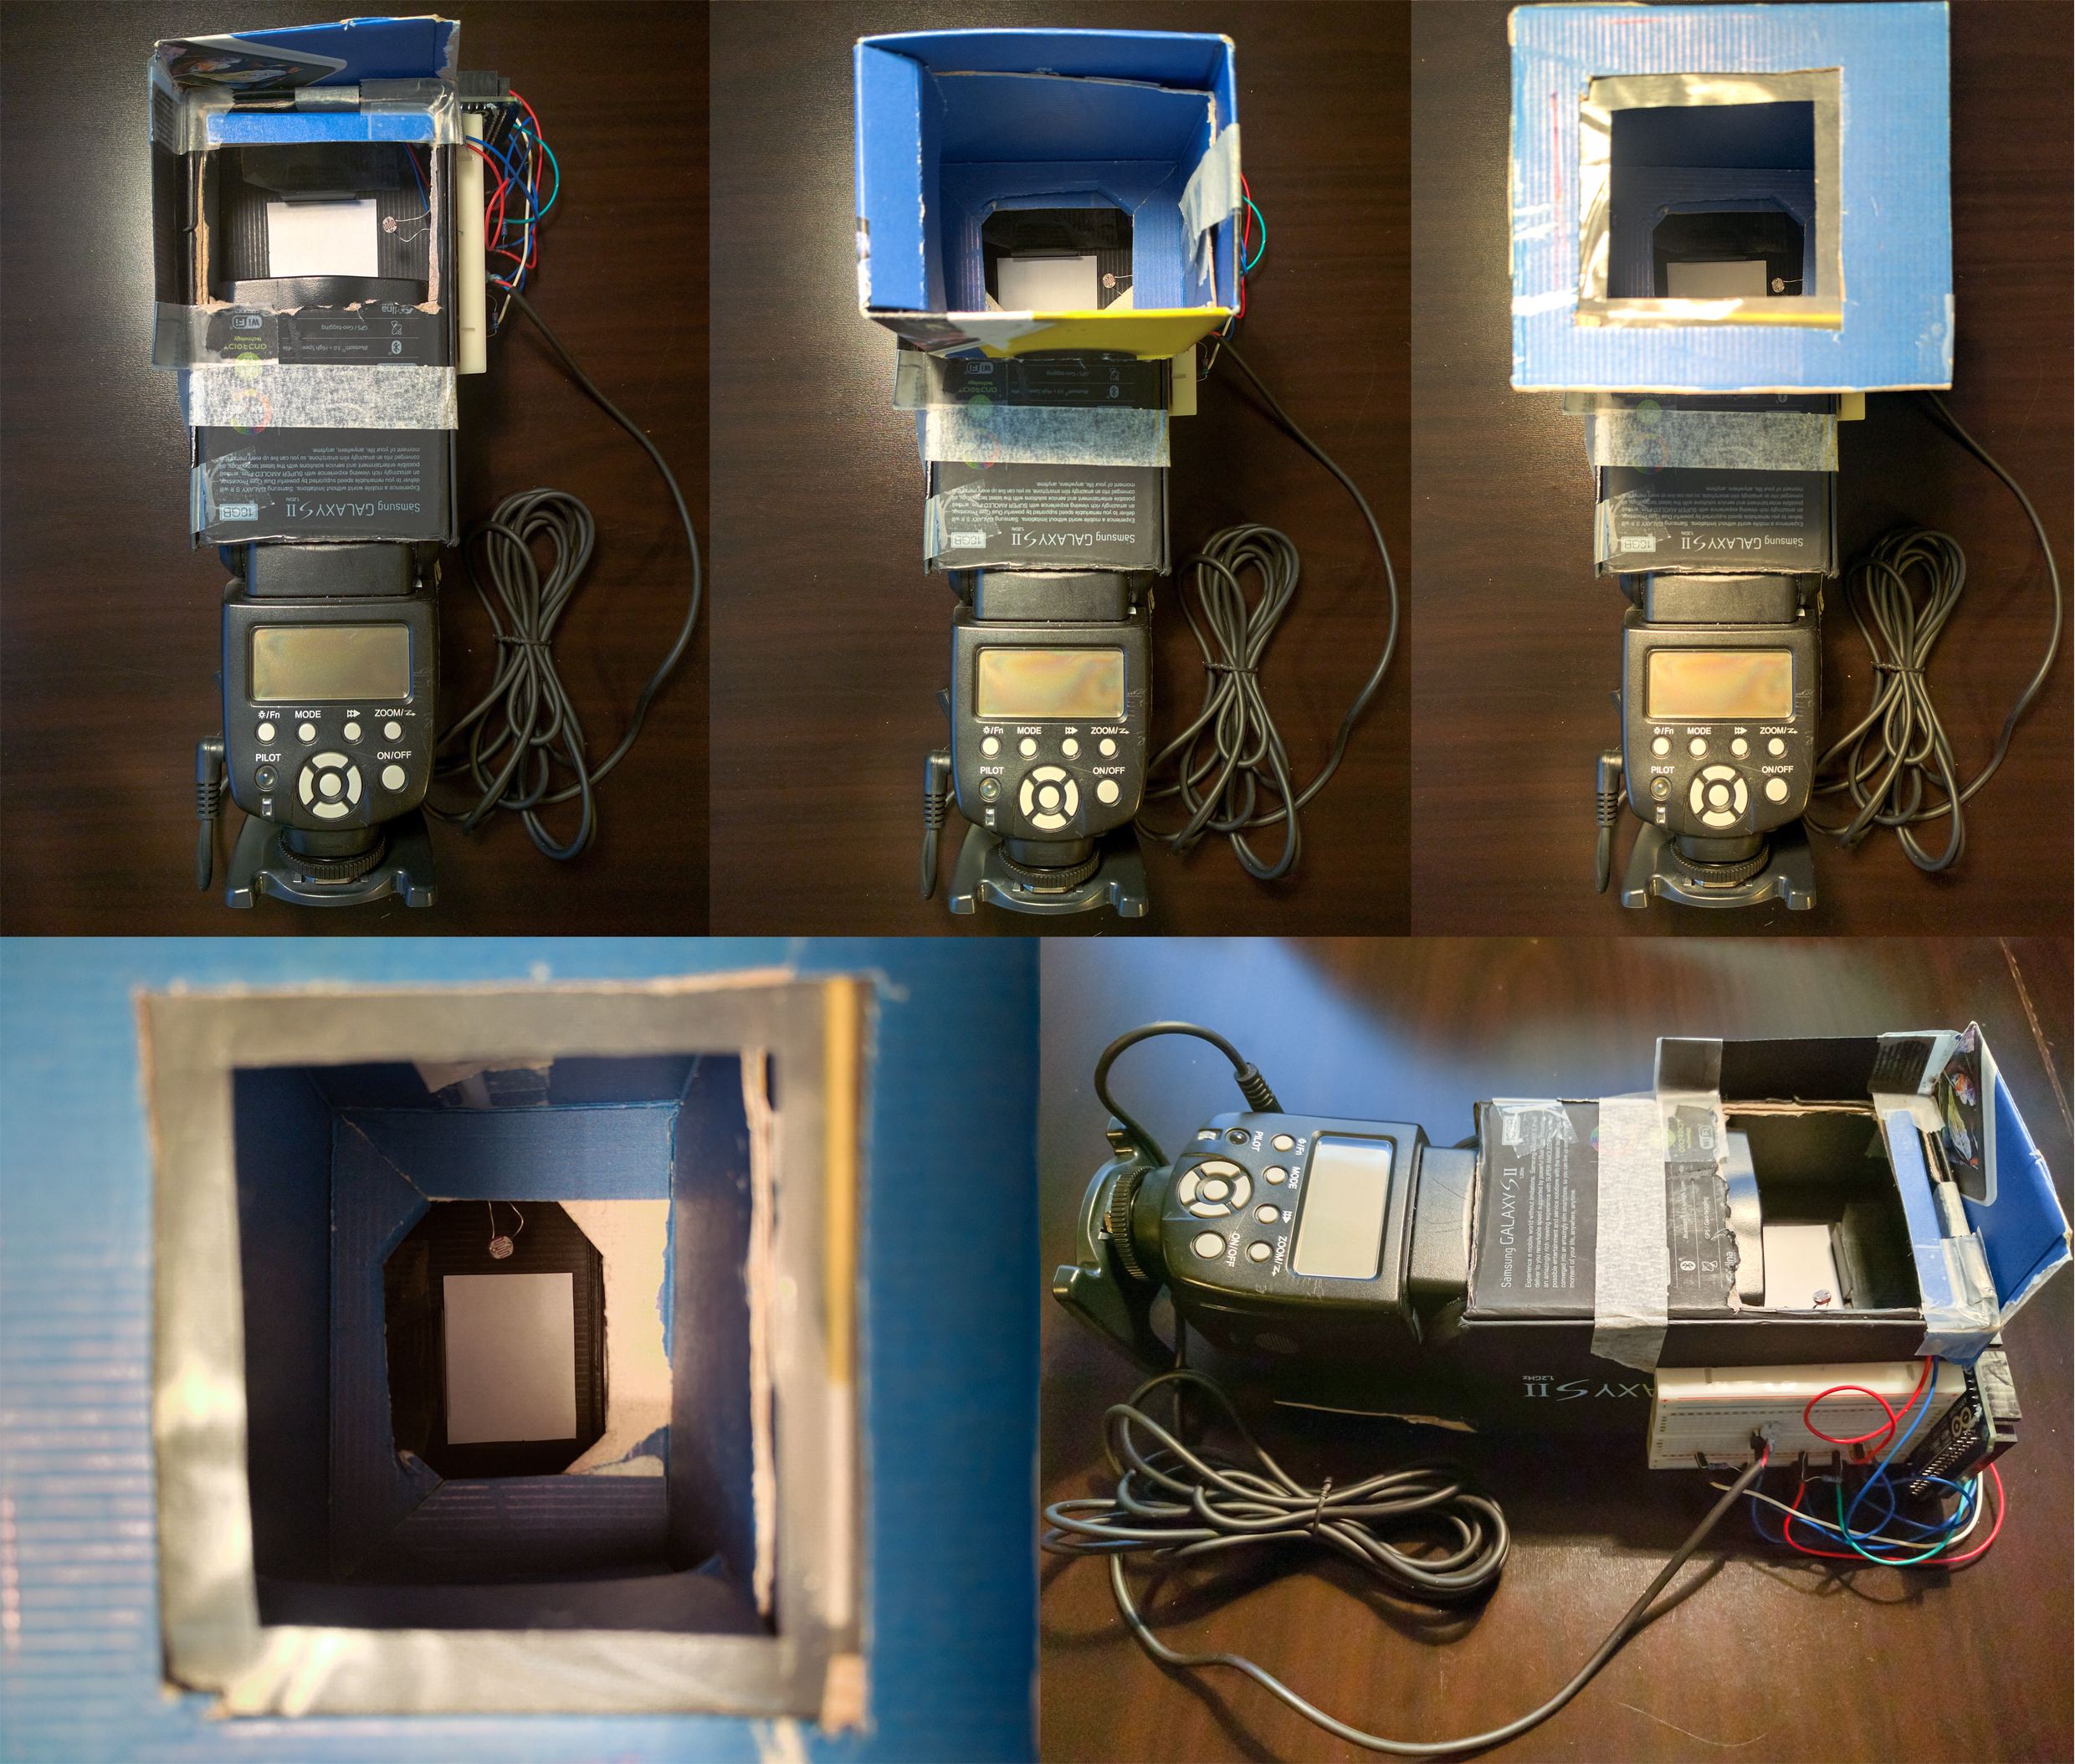
\includegraphics[width=\textwidth,height=\textheight,keepaspectratio=true]{images/design_implementation/camera-module-actual.jpg}
\end{figure}




\chapter{Microcontroller Schematics}
\label{appendix:camera-module-schematics}

The schematics for the external camera module featuring an Arduino Mega 2560 microcontroller. An optocoupler (4N35) is used to safely isolate the external light source from the rest of the circuit.

\begin{figure}[h]
\centering 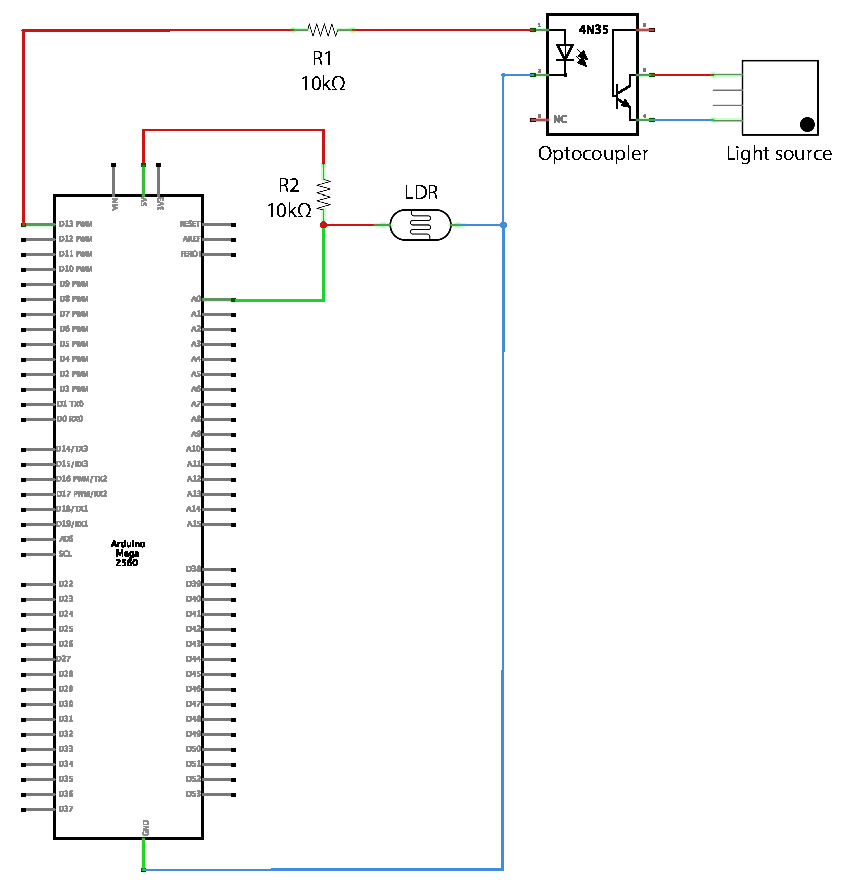
\includegraphics[width=12cm]{images/design_implementation/arduino_schematics.pdf}
\end{figure}





\chapter{Microcontroller Program (Arduino)}
\label{appendix:microcontroller-program}

The code utilizes Simon Monk's Arduino Timer library (version 1.3) \cite{arduino_timer_library}.

\lstinputlisting[language=C++,caption={main.ino}]{../app/camera-module/arduino/code/code.ino}

\lstinputlisting[language=C++,caption={is\_focused.ino}]{../app/camera-module/arduino/code/is_focused.ino}

\end{document}